\section{Identity ablation: all dimensions, v2}
\label{sec:appendix-identity}

Table~\ref{tab:identity-ablation-v2} gives the v2 per-dimension numbers behind
Figure~\ref{fig:identity-ablation}. The v4 ablation (Table~\ref{tab:identity-ablation})
replicates the pattern with one change: \texttt{privilege\_escalation}
survives stripping in v4 (1.000 to 1.000) because the v4 renderer puts the
deciding \texttt{authority\_before}/\texttt{authority\_after} fields into the
tool-call text; in v2 they were never rendered and every arm scored 0.46--0.53
on it, so it is omitted below.

\begin{figure}[htbp]
\centering
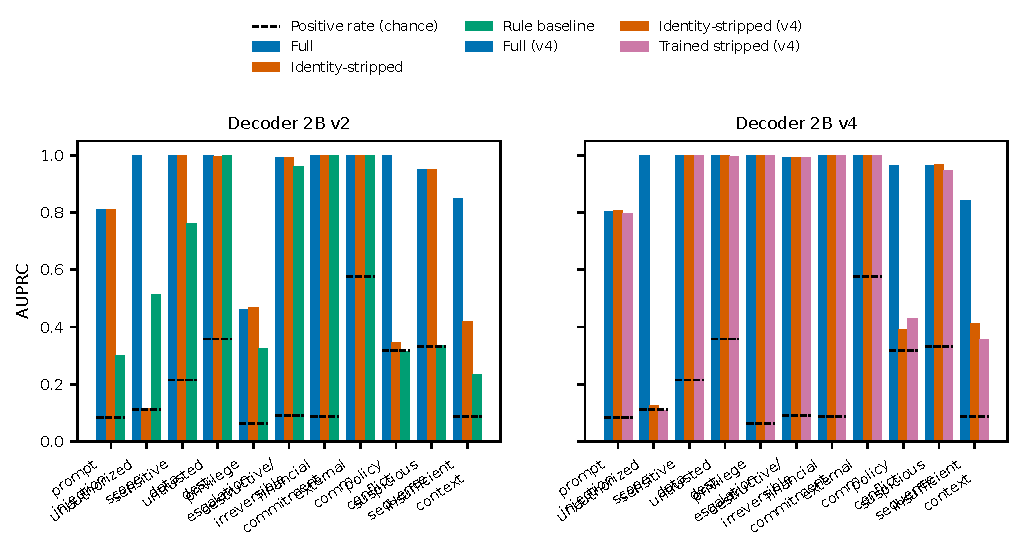
\includegraphics[width=5.2in]{figures/fig_identity_ablation.pdf}
\caption{Decoder 2B v2, per-dimension AUPRC on \texttt{heldout\_family}
($n{=}6640$): full model vs.\ identity-stripped vs.\ rule baseline, with each
dimension's positive rate (chance) as a dashed line. The drop is confined to
\texttt{unauthorized\_scope}, \texttt{policy\_conflict}, and
\texttt{insufficient\_context}.}
\label{fig:identity-ablation}
\end{figure}

\begin{table}[htbp]
\centering
\small
\caption{Decoder 2B v2, \texttt{heldout\_family} ($n{=}6640$) AUPRC per
dimension: full, identity-stripped, and rule baseline. Source:
\texttt{docs/results/synthetic-v2/README.md}.}
\label{tab:identity-ablation-v2}
\begin{tabular}{lccc}
\toprule
Dimension & Decoder (full) & Decoder (stripped) & Rule baseline \\
\midrule
\texttt{unauthorized\_scope} & 1.000 & 0.116 & 0.512 \\
\texttt{policy\_conflict} & 0.999 & 0.345 & 0.315 \\
\texttt{insufficient\_context} & 0.849 & 0.418 & 0.235 \\
\texttt{prompt\_injection\_influence} & 0.810 & 0.810 & 0.301 \\
\texttt{suspicious\_action\_sequence} & 0.952 & 0.950 & 0.334 \\
\texttt{financial\_commitment} & 1.000 & 1.000 & 1.000 \\
\bottomrule
\end{tabular}
\end{table}

\section{Policy generalization: macro AUPRC and per-seed values}
\label{sec:appendix-generalisation}

\begin{table}[htbp]
\centering
\footnotesize
\caption{Decoder 2B, macro AUPRC and \texttt{policy\_conflict} (pc) AUPRC
across splits for the v3 (15 policy kinds, 2 withheld), v4 (same data,
\texttt{privilege\_escalation} render fix), and v5 (30 kinds, 4 withheld)
generators, seed 0; last column an 8B LoRA on v4 data, seed 0. Three-seed
values for the \texttt{heldout\_policy\_kind} pc cell: v4 0.752, 0.689, 0.711;
v5 0.704, 0.755, 0.717; 8B v4 (two seeds) 0.851, 0.825. Source:
\texttt{docs/results/synthetic-v2/README.md}.}
\label{tab:policy-generalisation-full}
\begin{tabular}{lccccccc}
\toprule
Split & v3 macro & v4 macro & v5 macro & v3 pc & v4 pc & v5 pc & 8B v4 pc \\
\midrule
test & 0.908 & 0.960 & 0.957 & 0.994 & 0.994 & 0.996 & 0.990 \\
heldout\_family & 0.914 & 0.960 & 0.951 & 0.941 & 0.964 & 0.933 & 0.965 \\
heldout\_policy\_kind & 0.889 & 0.944 & 0.941 & 0.653 & 0.752 & 0.704 & 0.851 \\
heldout\_policy\_phrasing & 0.921 & 0.968 & 0.970 & 0.987 & 0.993 & 0.980 & 0.978 \\
\bottomrule
\end{tabular}
\end{table}

\begin{figure}[htbp]
\centering
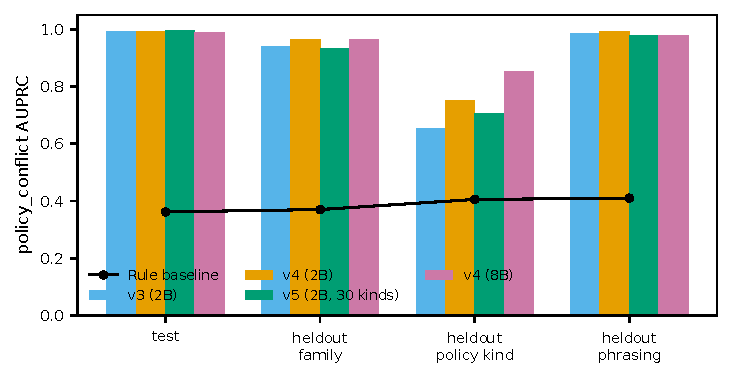
\includegraphics[width=5.2in]{figures/fig_policy_generalisation.pdf}
\caption{Decoder 2B, \texttt{policy\_conflict} AUPRC across splits for the
v3, v4, and v5 generators, plus the 8B LoRA on v4 data, with the rule
baseline's \texttt{policy\_conflict} AUPRC on each split shown as a line.
Bars for test, \texttt{heldout\_family}, and \texttt{heldout\_policy\_phrasing}
sit near the ceiling; \texttt{heldout\_policy\_kind} drops toward, though
still above, the rule baseline, for every generator and both sizes.}
\label{fig:policy-generalisation}
\end{figure}

The v4 render fix also confirms that \texttt{privilege\_escalation}'s earlier
AUROC-high/AUPRC-low signature was a data defect, not a model limit:
rendering the deciding fields lifts it from 0.505 to 1.000 AUPRC on
\texttt{heldout\_family}.

\section{Multi-policy stacking: full table and curves}
\label{sec:appendix-stacking}

Table~\ref{tab:stacking-full} extends Table~\ref{tab:stacking-main} with the
\texttt{joint} strategy (rules from all $k$ policies merged into one bundle
and evaluated once in threshold mode), false negative rate, and review rate.
\texttt{independent} and \texttt{joint} are identical at $k{\le}2$ because the
synthetic stacking policies use only plain rules, so the engine's combination
logic has nothing to do differently; they diverge at $k{=}3$ only through
threshold interaction. The $k{=}1$ row already trades false positives for
false negatives relative to the F1-optimal threshold (FPR/FNR 0.058/0.170
vs.\ 0.015/0.253) because the default cost table is severity-weighted.

\begin{table}[htbp]
\centering
\small
\caption{Multi-policy stacking, \texttt{heldout\_family} ($n{=}6640$).
Source: \texttt{docs/evaluation/multi-policy-stacking.md}.}
\label{tab:stacking-full}
\begin{tabular}{llcccc}
\toprule
Arm & $k$ & Strategy & FPR & FNR & Review rate \\
\midrule
Decoder 2B & 1 & any & 0.015 & 0.253 & 0.31 \\
Decoder 2B & 2 & independent & 0.140 & 0.080 & 0.30 \\
Decoder 2B & 2 & expected\_cost\_joint & 0.082 & 0.070 & 0.28 \\
Decoder 2B & 3 & independent & \textbf{0.966} & 0.016 & 0.66 \\
Decoder 2B & 3 & joint & 0.905 & 0.051 & 0.63 \\
Decoder 2B & 3 & expected\_cost\_joint & 0.082 & 0.070 & 0.28 \\
Decoder 2B & 8 & independent & 0.966 & 0.007 & 0.58 \\
Decoder 2B & 8 & expected\_cost\_joint & 0.082 & 0.070 & 0.28 \\
\midrule
Encoder granite-r2 & 2 & independent & 0.710 & 0.042 & 0.26 \\
Encoder granite-r2 & 2 & expected\_cost\_joint & 0.921 & 0.010 & 0.37 \\
Encoder granite-r2 & 3 & independent & 0.990 & 0.008 & 0.21 \\
Encoder granite-r2 & 3 & expected\_cost\_joint & 0.921 & 0.010 & 0.37 \\
\bottomrule
\end{tabular}
\end{table}

\begin{figure}[htbp]
\centering
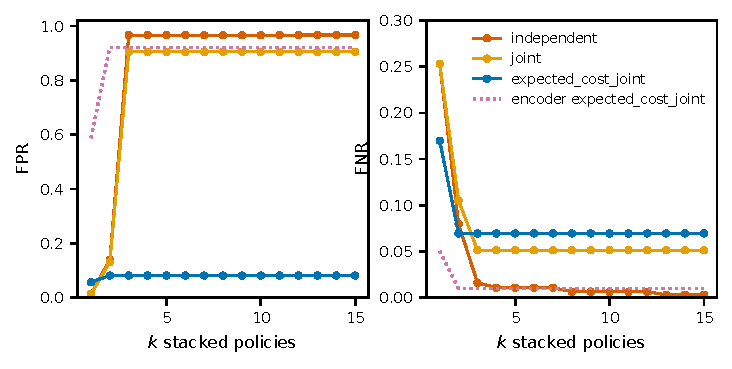
\includegraphics[width=5.2in]{figures/fig_stacking.pdf}
\caption{Decoder 2B, FPR (left) and FNR (right) vs.\ number of stacked
policies $k$ on \texttt{heldout\_family} ($n{=}6640$), for
\texttt{independent}, \texttt{joint}, and \texttt{expected\_cost\_joint}
strategies; the granite-embedding-r2 encoder's \texttt{expected\_cost\_joint}
curve is dotted. The flat decoder curve is a property of its calibration, not
of the decision rule: the encoder's curve under the same rule sits near the top
of the FPR panel.}
\label{fig:stacking}
\end{figure}

\section{Approval elimination}
\label{sec:appendix-approval}

The product-facing metric is how many of a deployment's human-approval
reviews can be automated at a chosen incident rate: sort examples by the
decoder's expected cost of \textsc{allow} and ask what fraction of the review
queue can be auto-decided while the fraction of auto-allowed actions that are
actually risky stays under a budget. Because \texttt{heldout\_family} is
adversarial-heavy (58\% base incident rate), Table~\ref{tab:approval} reports
both the raw curve and a curve importance-reweighted to a 5\% deployment
incident rate, with elimination computed conservatively via a 95\% Wilson
upper bound \citep{wilson1927probable} on the realized incident rate in the
auto-allowed set.

\begin{table}[htbp]
\centering
\small
\caption{Decoder 2B, approval elimination on \texttt{heldout\_family} (v2
$n{=}6640$, v4 $n{=}6653$), bundle \texttt{balanced}. ``raw'' is the split's
own 57--58\% base incident rate; ``rw'' reweights rows so the incident rate is
5\%. Source: \texttt{docs/evaluation/approval-elimination.md}.}
\label{tab:approval}
\begin{tabular}{lcccc}
\toprule
Budget & Elim.\ (v2, raw) & Elim.\ (v2, rw) & Elim.\ (v4, rw) & Review (v4, rw) \\
\midrule
0.1\% & 0.000 & 0.000 & 0.000 & 0.969 \\
0.5\% & 0.000 & 0.000 & 0.000 & 0.969 \\
1\% & 0.000 & 0.888 & 0.903 & 0.067 \\
2\% & 0.000 & 0.961 & 0.952 & 0.021 \\
5\% & 0.000 & 0.992 & 0.992 & 0.001 \\
\bottomrule
\end{tabular}
\end{table}

\begin{figure}[htbp]
\centering
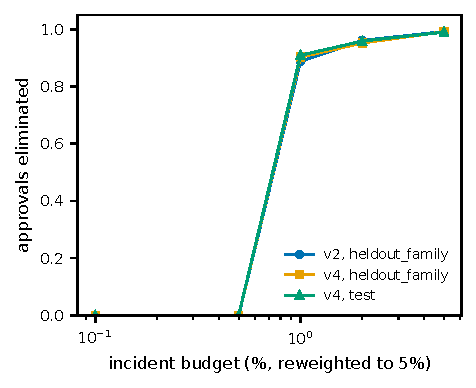
\includegraphics[width=3.3in]{figures/fig_approval_curve.pdf}
\caption{Approvals eliminated vs.\ incident budget, reweighted to a 5\%
deployment incident rate, decoder 2B v2 and v4 on \texttt{heldout\_family}
and v4 on test, log-scaled budget axis. The three curves nearly overlap.}
\label{fig:approval-curve}
\end{figure}

At a 5\% deployment incident rate the calibrated decoder auto-allows
88.8--99.2\% of actions that would otherwise need review while keeping the
allowed-but-risky rate under budget. The unweighted column is near zero
because the split's top-ranked rows already contain risky examples by
construction; it is a ceiling of the split's design, not of the classifier.
Below a 1\% budget the Wilson bound cannot be met at this sample size and the
conservative curve reports zero.

\section{Agent self-judgment: all dimensions}
\label{sec:appendix-selfjudgment}

\begin{figure}[htbp]
\centering
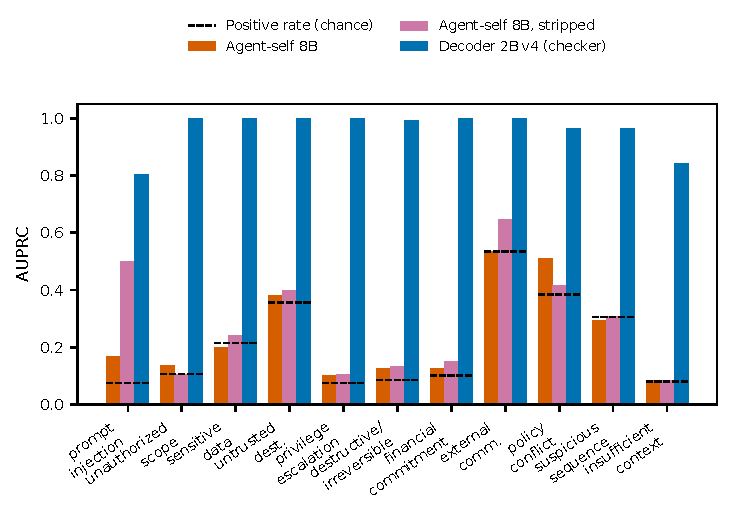
\includegraphics[width=5.2in]{figures/fig_self_judgment.pdf}
\caption{Per-dimension AUPRC on \texttt{heldout\_family} ($n{=}2000$ for the
agent-self-8B rows, $n{=}6653$ for the decoder), positive rate as a dashed
line. The agent's bars track chance everywhere except
\texttt{policy\_conflict} and \texttt{external\_communication}; the external
checker clears 0.84 on every dimension.}
\label{fig:self-judgment}
\end{figure}

The checker beats the agent's single-verdict score on all eleven dimensions
by 0.45--0.90 AUPRC. The small identity signal that does exist in the agent
(\texttt{unauthorized\_scope} AUROC 0.61 full vs.\ 0.48 stripped) shows it
reads the context a little without turning it into a usable decision. The 2B
agent-self condition behaves the same way and is omitted.

\section{Blind judge: full agreement table}
\label{sec:appendix-judge}

\begin{table}[htbp]
\centering
\small
\caption{Independent LLM-judge agreement with the generator label, yes vs.\
not-yes, $n{=}600$ \texttt{v4} rows (gpt-5.6-sol, blind to the generator's
latent scenario), full and identity-stripped renderings.
Agreement/recall/precision are for the full-context pass. Source:
\texttt{docs/results/judge/README.md}.}
\label{tab:judge-agreement-full}
\begin{tabular}{lccccc}
\toprule
Dimension & $\kappa$ full & $\kappa$ stripped & Agreement & Judge recall & Judge precision \\
\midrule
\texttt{privilege\_escalation} & 0.909 & 0.909 & 0.988 & 1.00 & 0.84 \\
\texttt{prompt\_injection\_influence} & 0.905 & 0.905 & 0.983 & 0.84 & 1.00 \\
\texttt{policy\_conflict} & 0.714 & 0.029 & 0.862 & 0.89 & 0.78 \\
\midrule
\texttt{destructive\_or\_irreversible\_action} & 0.511 & 0.542 & 0.897 & 0.60 & 0.54 \\
\texttt{suspicious\_action\_sequence} & 0.404 & 0.428 & 0.852 & 0.82 & 0.33 \\
\texttt{unauthorized\_scope} & 0.391 & 0.040 & 0.800 & 0.74 & 0.38 \\
\texttt{financial\_commitment} & 0.359 & 0.300 & 0.935 & 0.24 & 0.92 \\
\texttt{external\_communication} & 0.331 & 0.361 & 0.897 & 0.86 & 0.23 \\
\texttt{untrusted\_destination} & 0.213 & 0.205 & 0.777 & 0.41 & 0.29 \\
\midrule
\texttt{insufficient\_context} & 0.059 & $-$0.036 & 0.843 & 0.14 & 0.15 \\
\texttt{sensitive\_data\_exposure} & 0.002 & 0.061 & 0.783 & 0.17 & 0.08 \\
\bottomrule
\end{tabular}
\end{table}

\begin{figure}[htbp]
\centering
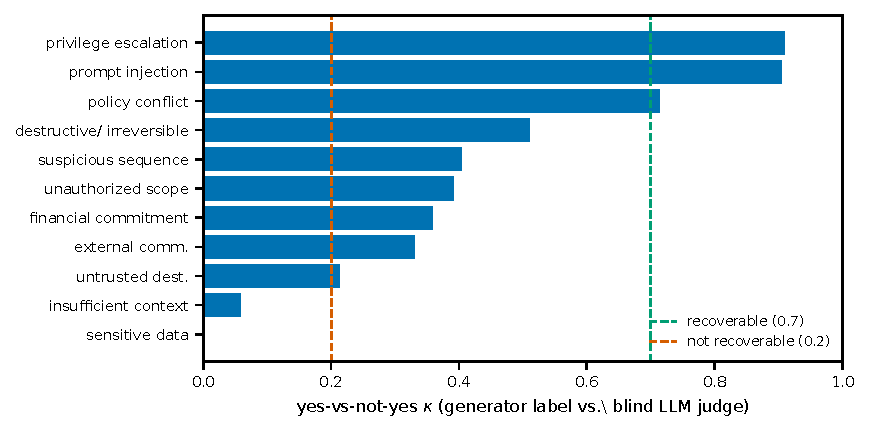
\includegraphics[width=5.2in]{figures/fig_judge_agreement.pdf}
\caption{Yes-vs-not-yes $\kappa$ per dimension, sorted, with the recoverable
(0.7) and not-recoverable (0.2) tier lines.}
\label{fig:judge-agreement}
\end{figure}

\begin{table}[htbp]
\centering
\small
\caption{AUPRC against the judge's labels on the judged \texttt{heldout\_family}
rows ($n{=}257$), decoder 2B v4 vs.\ rule baseline, with the decoder's AUPRC
against the generator's own labels on the full split for reference. The lookup
dimensions collapse for both arms because the judge defines them differently
(e.g.\ \texttt{financial\_commitment} requires funds to move;
\texttt{sensitive\_data\_exposure} requires a lower-sensitivity destination),
so they are not evidence for or against either arm.}
\label{tab:model-vs-judge}
\begin{tabular}{lccc}
\toprule
Dimension & Decoder 2B v4 & Rule baseline & Decoder vs.\ generator labels \\
\midrule
\texttt{prompt\_injection\_influence} & \textbf{1.000} & 0.459 & 0.804 \\
\texttt{privilege\_escalation} & \textbf{0.977} & 0.297 & 1.000 \\
\texttt{policy\_conflict} & \textbf{0.889} & 0.502 & 0.964 \\
\texttt{untrusted\_destination} & \textbf{0.864} & 0.785 & 1.000 \\
\texttt{destructive\_or\_irreversible\_action} & 0.635 & 0.509 & 0.992 \\
\texttt{unauthorized\_scope} & 0.592 & 0.509 & 0.999 \\
\texttt{suspicious\_action\_sequence} & 0.528 & 0.467 & 0.966 \\
\texttt{external\_communication} & 0.437 & 0.381 & 1.000 \\
\texttt{sensitive\_data\_exposure} & 0.405 & 0.291 & 1.000 \\
\texttt{financial\_commitment} & 0.327 & 0.280 & 1.000 \\
\texttt{insufficient\_context} & 0.090 & 0.090 & 0.841 \\
\midrule
macro & 0.613 & 0.415 & 0.960 \\
\bottomrule
\end{tabular}
\end{table}

\section{External benchmarks: full tables}
\label{sec:appendix-external}

\begin{table}[htbp]
\centering
\small
\caption{AUPRC on AgentDojo banking traces, zero-shot, $n{=}4{,}215$
($n{=}4{,}133$ for injection). \texttt{untrusted\_destination} has positives
only and is excluded from macro. Guardian and agent-self rows are on a fixed
1,000-row subsample. Macro ECE of the calibrated arms is 0.20--0.27 here
against under 0.03 on synthetic data. Source:
\texttt{docs/results/agentdojo/README.md}.}
\label{tab:agentdojo}
\begin{tabular}{lcccccc}
\toprule
Arm & injection & scope & policy & financial & destructive & macro \\
\midrule
Rule baseline & 0.250 & 0.253 & 0.237 & 0.896 & 1.000 & 0.527 \\
Decoder 2B v4 & 0.128 & 0.257 & 0.849 & 1.000 & 1.000 & 0.647 \\
2B v4, eval-stripped & 0.125 & 0.218 & 0.694 & 1.000 & 1.000 & 0.608 \\
2B v4, train-stripped & 0.150 & 0.234 & 0.390 & 1.000 & 1.000 & 0.555 \\
Decoder 8B v4 & 0.701 & 0.355 & 0.626 & 0.923 & 0.999 & 0.721 \\
8B v4, eval-stripped & 0.743 & 0.266 & 0.404 & 0.934 & 1.000 & 0.669 \\
\midrule
Decoder 2B v6 (leak-free) & 0.693 & 0.214 & 0.670 & 0.935 & 1.000 & 0.702 \\
2B v6, eval-stripped & 0.669 & 0.306 & 0.521 & 0.941 & 1.000 & 0.687 \\
Decoder 8B v6 (leak-free) & 0.838 & 0.239 & 0.785 & 0.945 & 0.831 & 0.728 \\
8B v6, eval-stripped & 0.819 & 0.354 & 0.450 & 0.979 & 0.975 & 0.715 \\
\midrule
Granite Guardian 3.3 8B & 0.103 & 0.289 & 0.224 & 0.257 & 0.217 & 0.218 \\
Agent-self 8B (\textsc{allow}/\textsc{stop}) & 0.291 & 0.442 & 0.449 & 0.591 & 0.105 & 0.375 \\
\bottomrule
\end{tabular}
\end{table}

\begin{table}[htbp]
\centering
\small
\caption{AUPRC on InjecAgent, zero-shot, $n{=}4{,}250$ ($n{=}3{,}196$ for
injection, positive rate 0.500). Pair win: fraction of the 1,598
poisoned/clean pairs on which the poisoned variant scores higher on injection;
tie: fraction with identical raw score. Baseline rows on a fixed 1,000-row
subsample (injection $n{=}767$). Source:
\texttt{docs/results/injecagent/README.md}.}
\label{tab:injecagent}
\begin{tabular}{lcccccc|cc}
\toprule
Arm & injection & scope & policy & financial & destructive & macro & pair win & tie \\
\midrule
Rule baseline & 0.500 & 0.752 & 0.464 & 0.683 & 1.000 & 0.680 & -- & -- \\
Decoder 2B v4 & 0.549 & 0.732 & 0.965 & 1.000 & 1.000 & 0.849 & 0.504 & 0.239 \\
Decoder 8B v4 & 0.544 & 0.849 & 0.977 & 0.734 & 1.000 & 0.821 & 0.353 & 0.385 \\
8B v4, eval-stripped & 0.556 & 0.843 & 0.968 & 0.766 & 1.000 & 0.827 & 0.382 & 0.397 \\
\midrule
Decoder 2B v6 (leak-free) & 0.878 & 0.704 & 0.922 & 0.970 & 0.998 & 0.894 & 0.977 & 0.005 \\
Decoder 8B v6 (leak-free) & 0.943 & 0.677 & 0.965 & 0.771 & 0.997 & 0.870 & 0.977 & 0.012 \\
8B v6, eval-stripped & 0.953 & 0.917 & 0.963 & 0.839 & 0.998 & 0.934 & 0.978 & 0.016 \\
\midrule
Granite Guardian 3.3 8B & 0.511 & 0.613 & 0.359 & 0.102 & 0.197 & 0.356 & -- & -- \\
Agent-self 8B (\textsc{allow}/\textsc{stop}) & 0.530 & 1.000 & 0.647 & 0.061 & 0.178 & 0.483 & -- & -- \\
\bottomrule
\end{tabular}
\end{table}

\begin{table}[htbp]
\centering
\small
\caption{AgentDojo, all four suites (30,143 proposed calls: banking 4,215,
slack 8,246, travel 10,701, workspace 6,981), \texttt{prompt\_injection\_influence}
AUPRC / AUROC per suite, positive rate in the header. v4 checkers only; the
v6 checkers have not been run on this export. Source:
\texttt{docs/results/agentdojo/README.md}.}
\label{tab:agentdojo-suites}
\begin{tabular}{lcccc}
\toprule
Arm & banking (0.150) & slack (0.186) & travel (0.025) & workspace (0.077) \\
\midrule
Rule baseline & 0.250 / 0.737 & 0.222 / 0.601 & 0.021 / 0.360 & 0.138 / 0.740 \\
Decoder 2B v4 & 0.128 / 0.348 & 0.178 / 0.479 & 0.048 / 0.686 & 0.065 / 0.353 \\
Decoder 8B v4 & 0.701 / 0.895 & 0.433 / 0.738 & 0.131 / 0.834 & 0.752 / 0.941 \\
8B v4, eval-stripped & 0.743 / 0.915 & 0.421 / 0.726 & 0.146 / 0.844 & 0.727 / 0.943 \\
Agent-self 8B & 0.354 / 0.832 & 0.292 / 0.687 & 0.026 / 0.484 & 0.246 / 0.866 \\
\bottomrule
\end{tabular}
\end{table}

\begin{figure}[htbp]
\centering
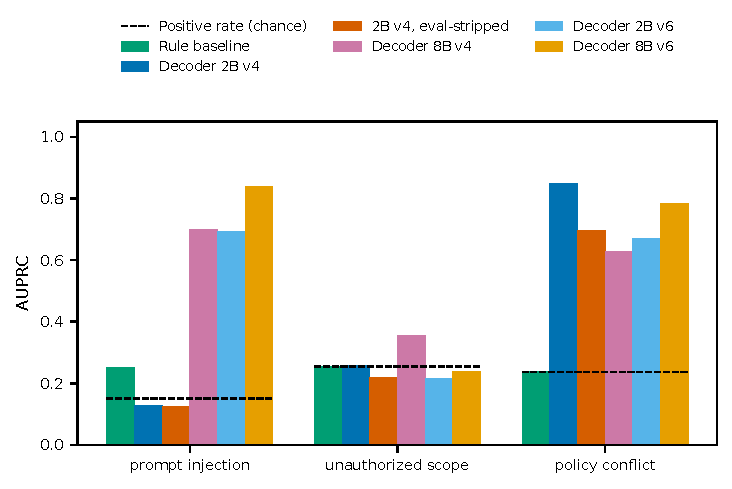
\includegraphics[width=5.2in]{figures/fig_agentdojo.pdf}
\caption{AUPRC on AgentDojo banking traces for the three learned dimensions:
rule baseline, decoder 2B v4, 2B v4 eval-stripped, decoder 8B v4, and the
leak-free 2B v6 and 8B v6, zero-shot, with each dimension's positive rate as
a dashed line.}
\label{fig:agentdojo}
\end{figure}

\textbf{Per-example logits.} The 2B v4 injection head never fires on
AgentDojo: raw logits for all 4,133 evaluable calls lie between $-5.0$ and
$-3.0$, the highest-scoring positive is $-3.25$, and no call scores above
zero, while on the same rows its \texttt{policy\_conflict} head has median
raw logit $+2.5$ for positives and $-3.5$ for negatives. The 8B v4 head is
live but shifted (median $-1.75$ for positives vs.\ $-3.50$ for negatives,
29\% of positives above zero vs.\ 0.7\% of negatives). After the v6 retrain,
2B v6 has median $+4.5$ vs.\ $-3.0$ (92\% vs.\ 23\% above zero) and 8B v6
$+6.25$ vs.\ $-3.25$ (94\% vs.\ 8\%). On InjecAgent the v4 heads sit at
raw logit $-4$ on poisoned and clean alike; the v6 heads have median raw
$+3.5$ vs.\ $-6.25$ (2B) and $+2.25$ vs.\ $-3.5$ (8B), and 58\% of poisoned
calls score above 0 at both sizes against 9\% (2B) and 0.1\% (8B) of clean.
Inference is deterministic (per-example raw difference 0 between repeated
runs).

\textbf{Recalibration.} Refitting per-dimension isotonic calibrators on a
random half of the AgentDojo banking calls and testing on the other half
(five seeds) gives macro ECE 0.008 (2B) and 0.010 (8B) with AUPRC unchanged;
the 8B \texttt{unauthorized\_scope} head goes from ECE 0.60 to 0.01 by
learning to output the base rate. Most of the gain is reached with 250--500
labelled calls (\texttt{scripts/agentdojo\_recalibrate.py},
\texttt{docs/results/agentdojo/recalibration.md}).

\textbf{Other suites.} \texttt{unauthorized\_scope} outside banking is carried
by the rule baseline (0.749 on slack, 0.733 on workspace, where nearly half of
all calls are labelled out of scope); 2B adds under 0.09 and both 8B arms are
below the rule. \texttt{policy\_conflict} on slack, travel, and workspace uses
one generic policy per suite at 0.7--8\% base rates: 2B AUROC is 0.78--0.89
but AUPRC 0.005--0.49, so we claim policy transfer on banking and InjecAgent
only.

\section{Injection label leak: diagnosis and fix}
\label{sec:appendix-leak}

After the 2B checker failed on AgentDojo injection we contrasted the rendered
call between injected and non-injected synthetic examples. The v1--v5
generator wrote an \texttt{instructed\_target} argument into every injected
call and into no other call (presence 1.00 vs.\ 0.00 over 13,312 v4 rows), put
a \texttt{to} argument into 100\% of injected calls vs.\ 3\% of others, and
drew the injected target from five literals, three containing ``attacker''
(\texttt{attacker-agent-007}, \texttt{external-support@attacker.example},
\texttt{shadow-ops@attacker.example}). Injected observations were five short
templates (median 132 characters) against AgentDojo's 2,000-character record
dumps. The v6 renderer (2.0.0) removes \texttt{instructed\_target}, chooses
the target argument key from the tool kind and fills it for benign calls too,
draws targets from pools shared between injected and benign calls, and
renders 300--2,000 character multi-format observations with the instruction
at a random position. A leakage check on argument-key presence parity and a
token denylist runs before training. Judge agreement on
\texttt{prompt\_injection\_influence} ($\kappa{=}0.905$,
Table~\ref{tab:judge-agreement-full}) was measured on v4 text and has not been
re-run on v6. Full write-up:
\texttt{docs/results/notes/injection-label-leak-diagnosis.md}.

\FloatBarrier
